% LTeX: language=fr

\chapter{Architecture de la solution d'analyse}

Avant d'aborder l'architecture de la solution d'analyse, il est important d'expliquer les raisons qui ont poussé à la création d'une solution d'analyse et les alternatives possibles.

D'abord, les trois possibilités pour effectuer des analyses forensiques et des analyses de malware sont:
\begin{enumerate}
    \item Analyser directement sur le PC de l'analyste. Il suffit d'installer les outils d'analyse directement dessus et lancer les analyses. C'est la solution de facilité parce que chaque analyste possède déjà sa propre machine et presque certainement la possibilité d'installer des outils d'analyse et de les lancer avec des droits administrateur le cas échéant. C'est aussi la solution la plus dangereuse car s'il survient le moindre incident sur cette machine, il faudra réinitialiser l'ordinateur, ce qui pourrait faire perdre plusieurs jours, voir semaines de travail. Mais il faudra aussi réinitialiser tous ses identifiants, et potentiellement investiguer les serveurs auxquels il avait accès si on trouve des traces de mouvement latéral dans l'entreprise.
    \item Une deuxième possibilité est d'utiliser un PC dédié à l'analyse forensique et de malware. Ça éviterait, lorsqu'on doit réinitialiser une machine compromise, les identifiants de l'utilisateur et, si elle n'a pas accès au réseau de l'entreprise, d'enquêter sur de potentiels mouvements latéraux. Il y a cependant des difficultés avec cette solution aussi, bien évidemment. Par exemple, si on oublie de la déconnecter du réseau, on risque à nouveau de contaminer d'autres machines dans l'entreprise. La seconde difficulté rencontrée est le nombre de PC d'analyse disponibles. En effet, s'il n'y en a qu'un, ça peut réduire la vitesse d'analyse lors des incidents et s'il y en a plusieurs, ça ajoute des coûts et du travail parce qu'il y a plus de machines à installer et mettre à jour.
    \item La dernière solution est l'utilisation d'une infrastructure isolée dans le cloud qui permet d'analyser les données tout en prévenant les mouvements latéraux. C'est la solution la plus sécurisée et la plus pratique parce qu'on peut créer des nouvelles machines à la demande et facilement les restaurer dans un état vierge à partir d'une snapshot (un instantané de la machine virtuelle, autrement dit une copie de la machine à un instant T). Le désavantage principal de cette solution est qu'on peut perdre beaucoup de temps pour transférer les données vers l'infrastructure isolée. En effet, on est dépendant du réseau, mais en plus, dans la plupart des infrastructures isolées, il faut passer par une sorte de \textit{jump host}, c'est-à-dire un intermédiaire sécurisé qui se trouve à la frontière entre le réseau isolé et l'extérieur. Évidemment, ajouter un intermédiaire ralentit le temps de transfert.
\end{enumerate}

La troisième solution a été choisie à la fois pour son isolation et pour son agilité. Malgré tout, dans les situations pratiques où il faut aller enquêter dans d'autres entreprises ou quand la situation est très urgente, avoir un PC d'analyse pour éviter de perdre du temps à transférer les données vers les machines virtuelles d'analyse dans le cloud est souhaitable. La deuxième solution reste donc très intéressante et est une voie d'amélioration que j'ai suggérée dans le rapport de stage.

Comme vous pouvez le voir sur la figure \ref{fig:architecture-sandboxing-simplified}, il y a plusieurs machines virtuelles installées dans le réseau isolé. Il y a la machine d'analyse SIFT/REMnux qui est la combinaison de SIFT et REMnux, une machine Linux basée sur Ubuntu. Elle contient la sandbox et peut donc lancer des machines virtuelles imbriquées pour analyser de manière dynamique les malwares qui lui sont soumis. La deuxième machine d'analyse est FLARE VM basée sur Windows. La dernière machine présente dans le réseau isolé est une sorte de \textit{jump host}. Mais contrairement à un jump host, elle ne sert pas à prendre contrôle d'une machine de haute importance comme un Domain Controller dans un domaine Active Directory, il sert d'intermédiaire entre les machines d'analyse qui peuvent être infectées lors de l'analyse de malware et l'extérieur. Toute cette infrastructure se trouve dans NECS, le cloud hybride de NRB.

\begin{figure}
    \centering
    \makebox[\textwidth]{
        \resizebox{15cm}{!}{
            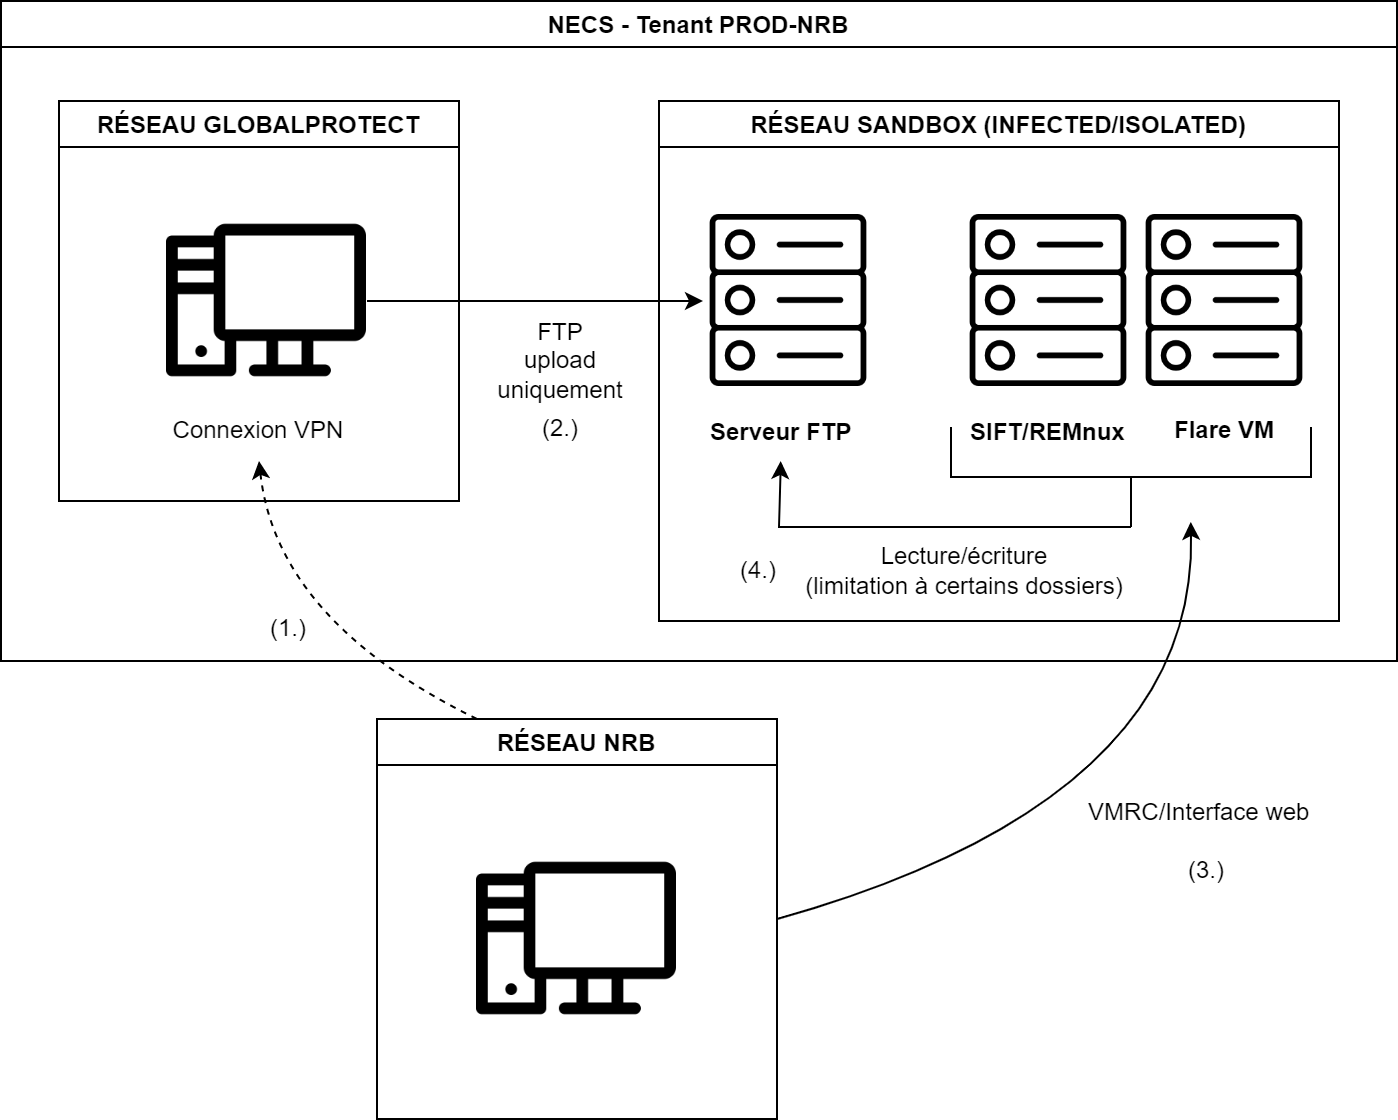
\includegraphics[width=0.95\linewidth]{images/infra-sandbox/infra-sandbox-simplified-01.png}
        }
    }
    \caption{Architecture simplifiée avec les étapes précédant l'analyse.}
    \label{fig:architecture-sandboxing-simplified}
\end{figure}

Avant de pouvoir lancer l'analyse d'un malware ou de données forensiques, il faut bien sûr amener les données sur les machines d'analyse en passant par le serveur FTP. Les quatre étapes à accomplir sont donc:

\begin{enumerate}
    \item Se connecter en VPN (avec le VPN GlobalProtect) sur le réseau NECS.
    \item Uploader les données vers le serveur FTP avec l'utilisateur \textit{upload}.
    \item Se connecter aux machines d'analyse via VMRC (VMWare Remote Console) ou l'interface web (NECS possède la possibilité d'accéder à l'interface graphique de la machine virtuelle via une interface web).
    \item Depuis la machine d'analyse, aller chercher les éléments à analyser en FTP.
\end{enumerate}

Le fait qu'il y ait autant d'étapes n'est pas un problème quand on veut effectuer une analyse forensique de temps à autre. Mais c'est une réelle contrainte si on veut seulement réaliser une analyse rapide et automatique de malware, surtout que ça peut arriver souvent. Puisque la plateforme d'analyse de malware FAME et la sandbox CAPE possèdent toutes les deux une interface web, une amélioration proposée est d'ouvrir le port 80 (le port HTTP) du réseau isolé vers le réseau utilisé lorsqu'on se connecte en VPN avec GlobalProtect. C'est cependant plus risqué d'un point de vue de la cybersécurité parce que le protocole HTTP est souvent utilisé par les malwares.

Évidemment, quand on crée un réseau isolé d'internet, on ne peut plus mettre à jour les machines qui s'y trouvent. Alors pour pouvoir quand même se connecter à internet et effectuer les mises à jour ou installer des nouveaux outils, il y a un deuxième réseau qui a été créé au sein du tenant: le réseau de management. Vous pouvez le voir sur la gauche de la figure \ref{fig:architecture-sandboxing}. L'idée initiale était qu'après l'installation des machines virtuelles, un template de la machine allait être créé afin de pouvoir en générer des nouvelles à volonté. Ensuite, quand on décide de faire une mise à jour, il suffit de recréer la machine à partir du template dans le réseau de management, réaliser les mises à jour et écraser le template avec cette nouvelle machine. Il y aurait toujours des snapshots de machines prêtes pour l'analyse dans le réseau isolé au cas où il faut lancer une analyse sans attendre. Mais les templates auraient été au cœur du système pour créer plusieurs machines lorsque plusieurs analystes doivent effectuer des analyses en même temps ou pour les mises à jour. Malheureusement, il y a eu des problèmes avec la création de templates parce que les machines d'analyse sont très spécifiques (par exemple: une Windows 10 au lieu d'une Windows Server), ce qui fait que pour faire les mises à jour, il faut d'abord restaurer la machine virtuelle à partir de sa snapshot, la déplacer dans le réseau de management avant de faire les mises à jour.

\begin{figure}
    \centering
    \makebox[\textwidth]{
        \resizebox{19cm}{!}{
            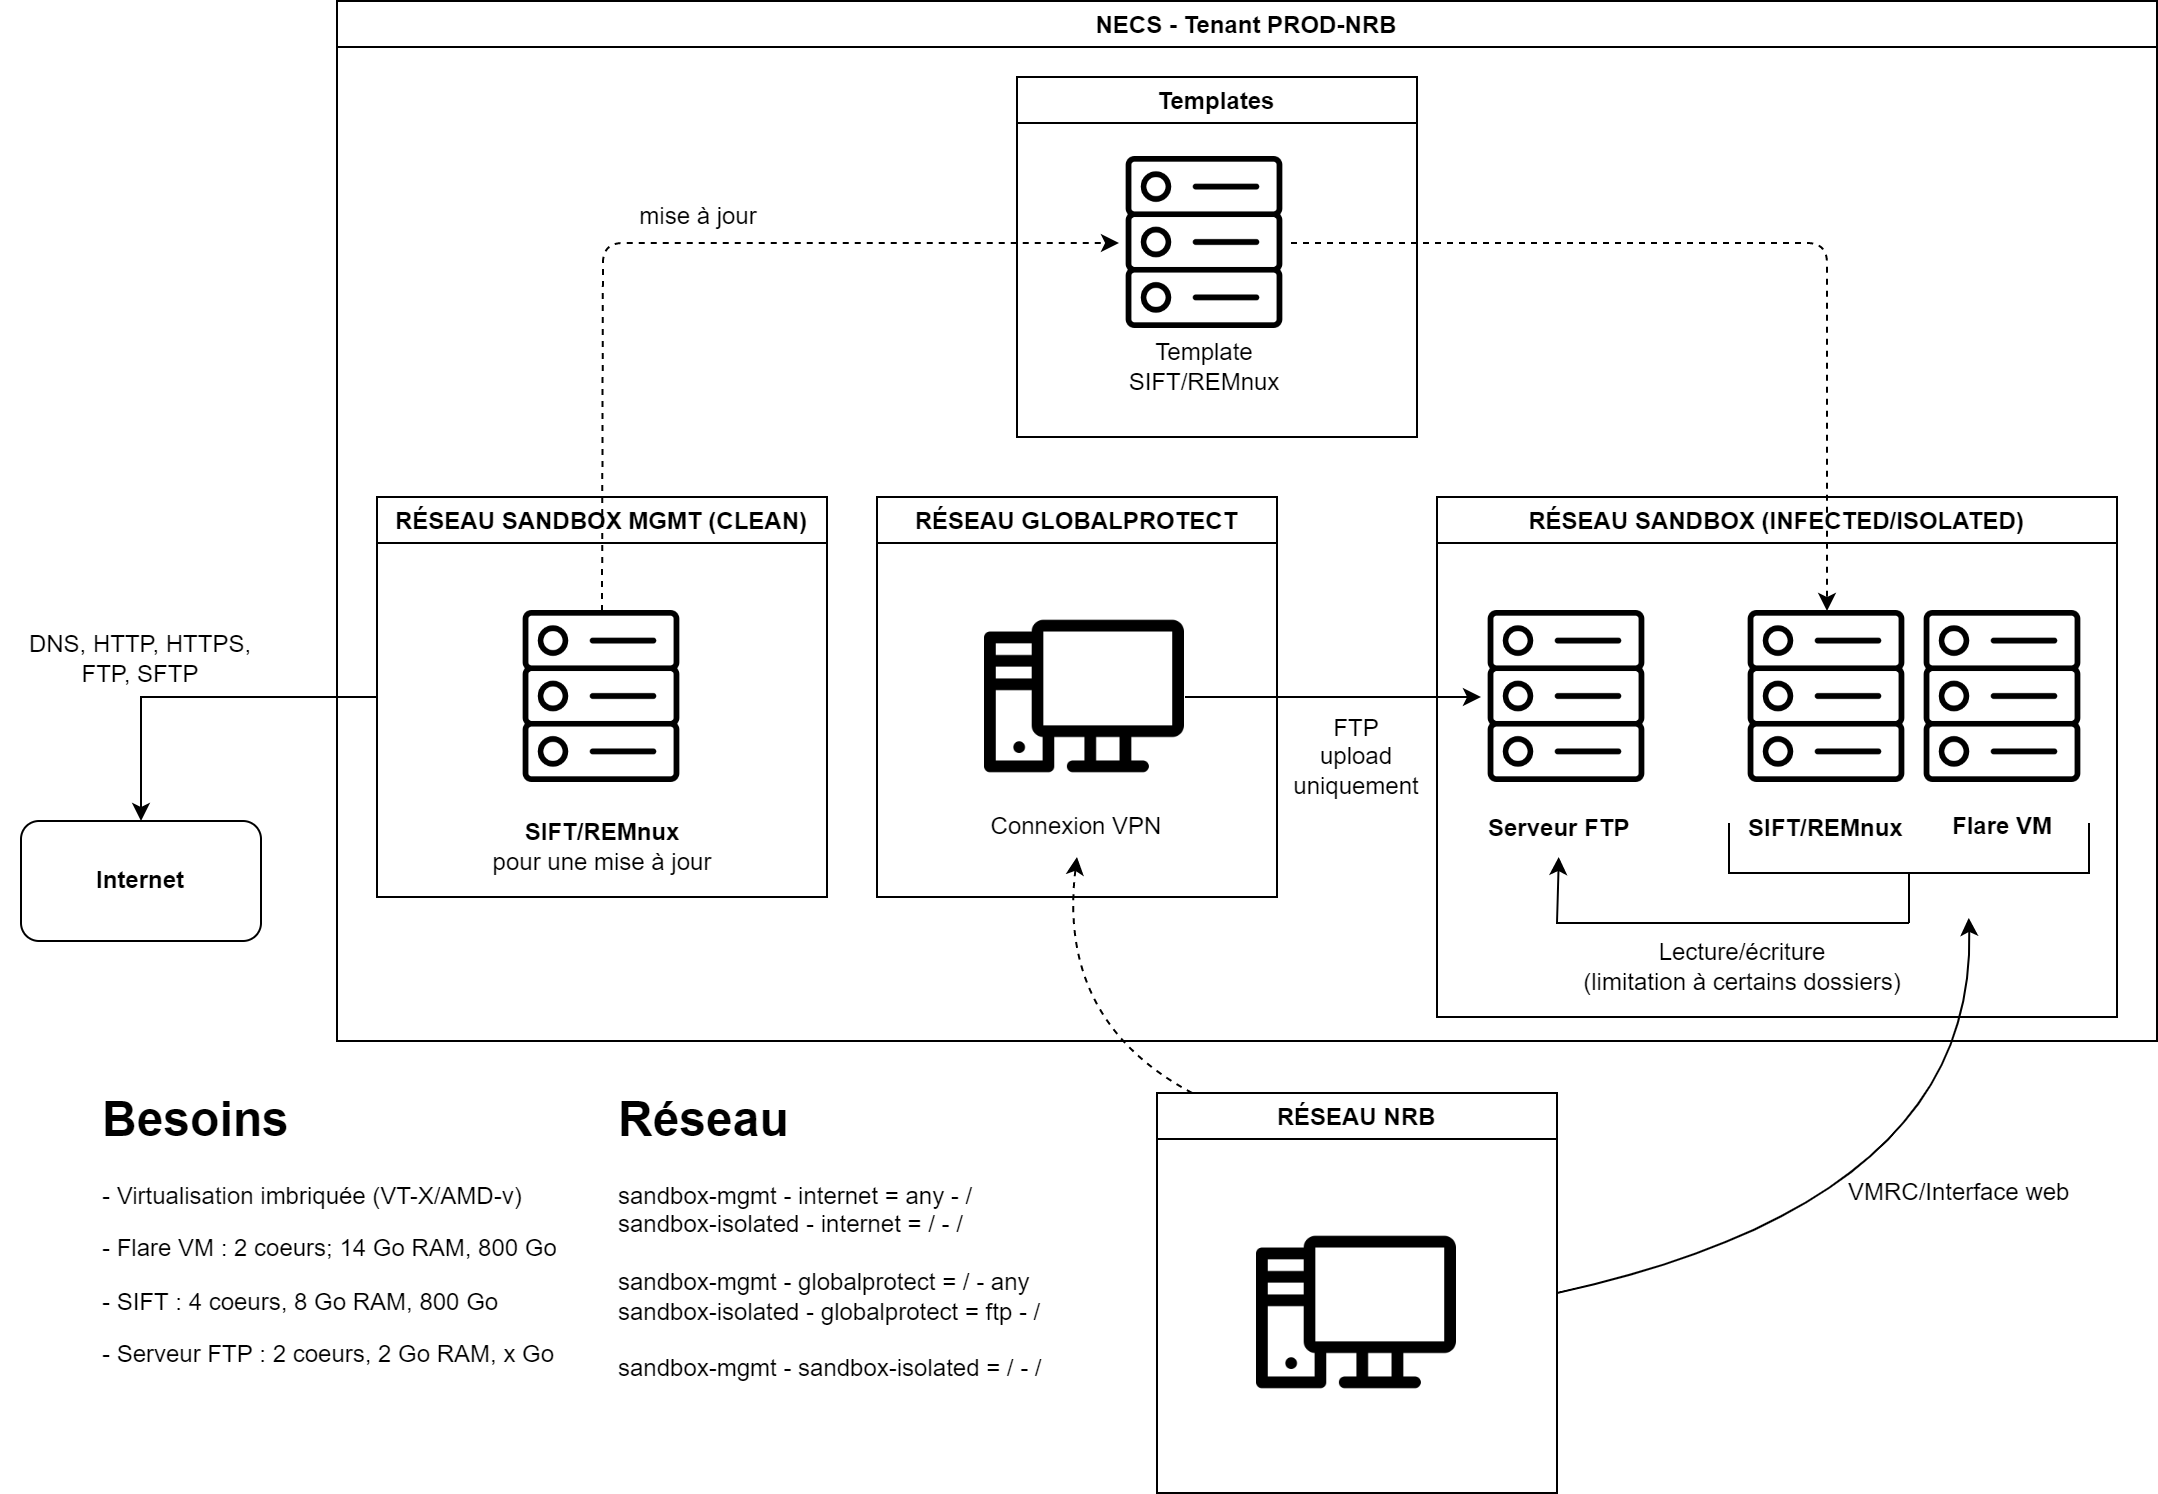
\includegraphics[width=0.95\linewidth]{images/infra-sandbox/infra-sandbox.png}
        }
    }
    \caption{Architecture de la solution d'analyse forensique et de malwares.}
    \label{fig:architecture-sandboxing}
\end{figure}

